%%%%%%%%%%%%%%%%%%%%%%%%%%%%%%%%%%%%%%%%%
% Beamer Presentation
% LaTeX Template
% Version 1.0 (10/11/12)
%
% This template has been downloaded from:
% http://www.LaTeXTemplates.com
%
% License:
% CC BY-NC-SA 3.0 (http://creativecommons.org/licenses/by-nc-sa/3.0/)
%
%%%%%%%%%%%%%%%%%%%%%%%%%%%%%%%%%%%%%%%%%

%----------------------------------------------------------------------------------------
%    PACKAGES AND THEMES
%----------------------------------------------------------------------------------------

\documentclass[aspectratio=169]{beamer}

\mode<presentation> {

\usetheme{CambridgeUS}

}

\usepackage{color}
\usepackage{graphicx} % Allows including images
\usepackage{url}
\usepackage{hyperref}
\usepackage{algorithm2e}
\usepackage{tikz}

\usetikzlibrary{automata,positioning,arrows,chains,fit,shapes}

\DontPrintSemicolon

\DeclareGraphicsExtensions{.png, .pdf}

\setlength{\parskip}{1em}

%----------------------------------------------------------------------------------------
%    TITLE PAGE
%----------------------------------------------------------------------------------------

\title[Complexity theory]{Complexity Theory} % The short title appears at the bottom of every slide, the full title is only on the title page

\author{Dominic Moylett} % Your name
\institute[University of Bristol] % Your institution as it will appear on the bottom of every slide, may be shorthand to save space
{
Quantum Engineering CDT\\
University of Bristol \\ % Your institution for the title page
\medskip
\textit{\href{mailto:dominic.moylett@bristol.ac.uk}{dominic.moylett@bristol.ac.uk}} % Your email address
}
\date{\today} % Date, can be changed to a custom date

\begin{document}

\begin{frame}
\titlepage % Print the title page as the first slide
\end{frame}

%----------------------------------------------------------------------------------------
%    PRESENTATION SLIDES
%----------------------------------------------------------------------------------------

\begin{frame}
\frametitle{Summary of Presentation}
This presentation will consist of two parts:
\begin{itemize}
	\item Part one will look at the building blocks of complexity classes
	\item And part two will look at the consequences of the complexity classes we defined
\end{itemize}

We'll finish by exploring other aspects of complexity theory, and giving examples of other complexity classes and open problems out there.
\end{frame}

%------------------------------------------------
\section{Introduction: What is complexity theory?}
%------------------------------------------------

\begin{frame}
\frametitle{Complexity theory in a nutshell}
\centerline{``How hard can it be?'', {\em Clarkson, Hammond, May}}
\end{frame}

\begin{frame}
\frametitle{What is complexity theory?}
Complexity theory is the study of what problems are easy to solve with a computer.
\end{frame}

\begin{frame}
\frametitle{What is complexity theory?}
Complexity theory is the study of what problems are {\color{red} easy} to solve with a computer.

How do we measure performance?
\end{frame}

\begin{frame}
\frametitle{What is complexity theory?}
Complexity theory is the study of what {\color{red} problems} are easy to solve with a computer.

What is a problem?
\end{frame}

\begin{frame}
\frametitle{What is complexity theory?}
Complexity theory is the study of what problems are easy to solve with a {\color{red} computer}.

What is a computer?
\end{frame}

\begin{frame}
\frametitle{Structure of part one}
\begin{itemize}
    \item What is a computer?
    \item What is a problem?
    \item How do we measure performance?
\end{itemize}
\end{frame}

%------------------------------------------------
\section{What is a computer?}
%------------------------------------------------

\begin{frame}
\frametitle{Our model of a computer}
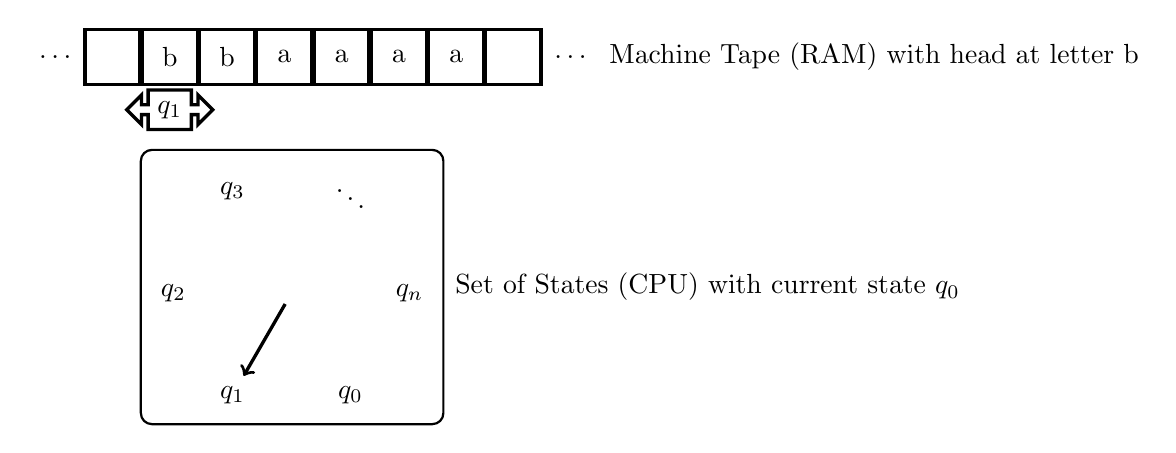
\begin{tikzpicture}
\tikzstyle{every path}=[very thick]

\edef\sizetape{0.7cm}
\tikzstyle{tmtape}=[draw,minimum size=\sizetape]
\tikzstyle{tmhead}=[arrow box,draw,minimum size=.5cm,arrow box
arrows={east:.25cm, west:0.25cm}]

%% Draw TM tape
\begin{scope}[start chain=1 going right,node distance=-0.15mm]
    \node [on chain=1,tmtape,draw=none] {$\ldots$};
    \node [on chain=1,tmtape] {};
    \node [on chain=1,tmtape] (input) {b};
    \node [on chain=1,tmtape] {b};
    \node [on chain=1,tmtape] {a};
    \node [on chain=1,tmtape] {a};
    \node [on chain=1,tmtape] {a};
    \node [on chain=1,tmtape] {a};
    \node [on chain=1,tmtape] {};
    \node [on chain=1,tmtape,draw=none] {$\ldots$};
    \node [on chain=1] {Machine Tape (RAM) with head at letter b};
\end{scope}

%% Draw TM Finite Control
\begin{scope}
[shift={(3cm,-3cm)},start chain=circle placed {at=(-\tikzchaincount*60:1.5)}]
\foreach \i in {q_0,q_1,q_2,q_3,\ddots,q_n}
    \node [on chain] {$\i$};

% Arrow to current state
\node (center) {};
\draw[->] (center) -- (circle-2);

\node[rounded corners,draw=black,thick,fit=(circle-1) (circle-2) (circle-3) 
      (circle-4) (circle-5) (circle-6),
            label=right:Set of States (CPU) with current state $q_0$] (fsbox)
        {};
\end{scope}

%% Draw TM head below (input) tape cell
\node [tmhead,yshift=-.3cm] at (input.south) (head) {$q_1$};

\end{tikzpicture}\footnote{\url{http://www.texample.net/tikz/examples/turing-machine-2/}}
\end{frame}

\begin{frame}
\frametitle{Formal definition of a computer}
A Turing Machine $(TM)$ is specified as a tuple of seven components $(Q, \Sigma, \Gamma, q_0, q_{accept}, q_{reject}, \delta)$:

\begin{itemize}
    \item<1-> $Q$ is the set of all possible states
    \item<2-> $\Sigma$ is the input alphabet for the tape. Note that $\Sigma$ cannot contain the blank symbol $\sqcup$
    \item<3-> $\Gamma$ is tape alphabet, where $\Sigma \subseteq \Gamma$ and $\sqcup \in \Gamma$
    \item<4-> $q_0 \in Q$ is the start state
    \item<5-> $q_{accept} \in Q$ is the accept state
    \item<6-> $q_{reject} \in Q$ is the reject state, where $q_{reject} \neq q_{accept}$
    \item<7-> $\delta: Q \times \Gamma \to Q \times \Sigma \times \{L, R\}$ is the transition function
\end{itemize}
\end{frame}

\begin{frame}
\frametitle{But how do we run it?}
The majority of computation time is spent repeating the following loop. Note that $T_h$ is the $h$-th cell of the tape.
\begin{algorithm}[H]
$q = q_0$\\
$h = 0$\\
$T = w$ \tcp*{Tape starts as just input, followed by blank cells}
\While{$q \notin \{q_{accept}, q_{reject}\}$}{
    $(q, T_h, i) = \delta(q, T_h)$\\
    \eIf{$i = L$}{$h = h - 1$ \tcp*{Move tape head to the left}}
    {$h = h + 1$ \tcp*{Move tape head to the right}}
}
\end{algorithm}
\end{frame}

\begin{frame}
\frametitle{What happens when it stops?}
When we reach either the {\em accept} or {\em reject} state, the machine has {\em halted}.

If $M$ halts in the accept state, then $M$ accepted the input.

If $M$ halts in the reject state, then $M$ rejected the input.
\end{frame}

\begin{frame}
\frametitle{What can we store in a machine's memory?}
\begin{itemize}
    \item<1-> Integers
    \item<2-> Rational numbers
    \item<3-> Floating point numbers
    \item<4-> Boolean (True/False) statements
    \item<5-> Text
    \item<6-> Graphs
    \item<7-> Other machines
\end{itemize}
\end{frame}

\begin{frame}
\frametitle{Universal Turing Machines}
Turing showed in his PhD thesis that we could represent any $TM$ after any number of transitions -- including current state, tape contents and position of tape head -- as an integer.

Not only that, but we could manipulate this integer such that it matched performing the next step of the computation.

This gave way to Universal Turing Machines; machines capable of running any $TM$ given to them.
\end{frame}

\begin{frame}
\frametitle{The Church-Turing Thesis}
\centerline{``[A]ll effectively calculable sequences are computable'', {\em Turing}}
\end{frame}

\begin{frame}
\frametitle{Quiz Time!}

\begin{center}
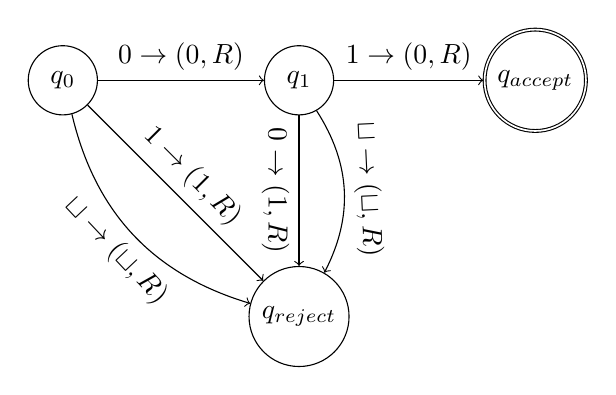
\begin{tikzpicture}[node distance=3cm,on grid,auto]
    \node[state] (q0) at (0,0) {$q_0$};
    \node[state] (q1) [right of=q0] {$q_1$};
    \node[accepting,state] (qaccept) [right of=q1] {$q_{accept}$};
    \node[state] (qreject) [below of=q1] {$q_{reject}$};
    \path[->]
        (q0) edge node {$0 \to (0, R)$} (q1)
        (q1) edge node {$1 \to (0, R)$} (qaccept)
        (q0) edge node[sloped, anchor=south] {$1 \to (1, R)$} (qreject)
        (q0) edge[bend right, sloped, anchor=north] node {$\sqcup \to (\sqcup, R)$} (qreject)
        (q1) edge node[sloped, anchor=north] {$0 \to (1, R)$} (qreject)
        (q1) edge[bend left, sloped, anchor=south] node {$\sqcup \to (\sqcup, R)$} (qreject);
\end{tikzpicture}
\end{center}

Question: Does $M$ accept or reject $01$?
\end{frame}

\begin{frame}[noframenumbering]
\frametitle{Quiz Time!}

\begin{center}
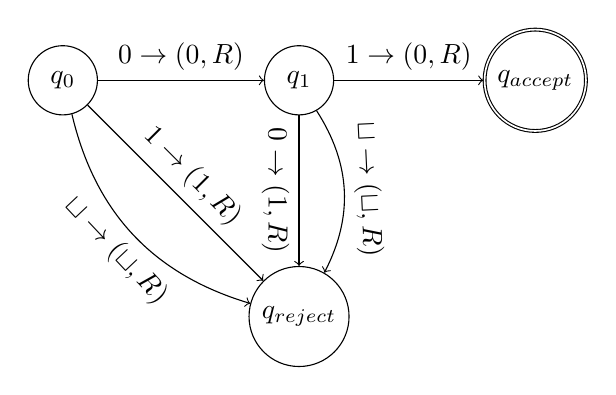
\begin{tikzpicture}[node distance=3cm,on grid,auto]
    \node[state] (q0) at (0,0) {$q_0$};
    \node[state] (q1) [right of=q0] {$q_1$};
    \node[accepting,state] (qaccept) [right of=q1] {$q_{accept}$};
    \node[state] (qreject) [below of=q1] {$q_{reject}$};
    \path[->]
        (q0) edge node {$0 \to (0, R)$} (q1)
        (q1) edge node {$1 \to (0, R)$} (qaccept)
        (q0) edge node[sloped, anchor=south] {$1 \to (1, R)$} (qreject)
        (q0) edge[bend right, sloped, anchor=north] node {$\sqcup \to (\sqcup, R)$} (qreject)
        (q1) edge node[sloped, anchor=north] {$0 \to (1, R)$} (qreject)
        (q1) edge[bend left, sloped, anchor=south] node {$\sqcup \to (\sqcup, R)$} (qreject);
\end{tikzpicture}
\end{center}

Answer: $M$ accepts $01$!
\end{frame}

\begin{frame}
\frametitle{Quiz Time!}

\begin{center}
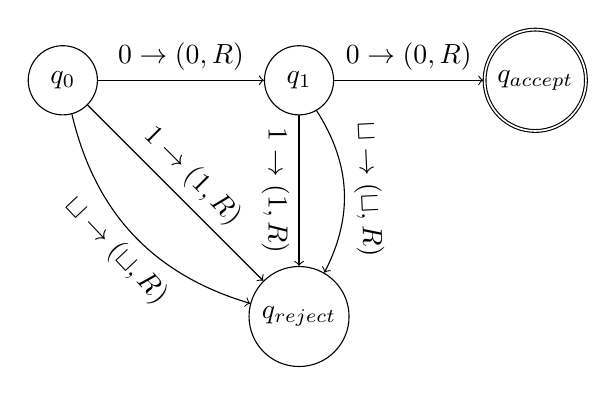
\begin{tikzpicture}[node distance=3cm,on grid,auto]
    \node[state] (q0) at (0,0) {$q_0$};
    \node[state] (q1) [right of=q0] {$q_1$};
    \node[accepting,state] (qaccept) [right of=q1] {$q_{accept}$};
    \node[state] (qreject) [below of=q1] {$q_{reject}$};
    \path[->]
        (q0) edge node {$0 \to (0, R)$} (q1)
        (q1) edge node {$0 \to (0, R)$} (qaccept)
        (q0) edge node[sloped, anchor=south] {$1 \to (1, R)$} (qreject)
        (q0) edge[bend right, sloped, anchor=north] node {$\sqcup \to (\sqcup, R)$} (qreject)
        (q1) edge node[sloped, anchor=north] {$1 \to (1, R)$} (qreject)
        (q1) edge[bend left, sloped, anchor=south] node {$\sqcup \to (\sqcup, R)$} (qreject);
\end{tikzpicture}
\end{center}

Question: Does $M$ accept or reject $01$?
\end{frame}

\begin{frame}[noframenumbering]
\frametitle{Quiz Time!}

\begin{center}
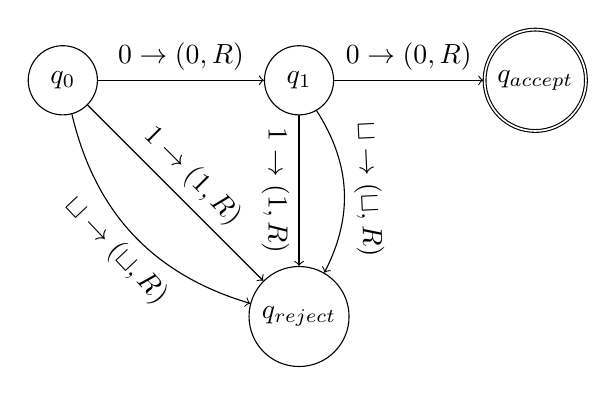
\begin{tikzpicture}[node distance=3cm,on grid,auto]
    \node[state] (q0) at (0,0) {$q_0$};
    \node[state] (q1) [right of=q0] {$q_1$};
    \node[accepting,state] (qaccept) [right of=q1] {$q_{accept}$};
    \node[state] (qreject) [below of=q1] {$q_{reject}$};
    \path[->]
        (q0) edge node {$0 \to (0, R)$} (q1)
        (q1) edge node {$0 \to (0, R)$} (qaccept)
        (q0) edge node[sloped, anchor=south] {$1 \to (1, R)$} (qreject)
        (q0) edge[bend right, sloped, anchor=north] node {$\sqcup \to (\sqcup, R)$} (qreject)
        (q1) edge node[sloped, anchor=north] {$1 \to (1, R)$} (qreject)
        (q1) edge[bend left, sloped, anchor=south] node {$\sqcup \to (\sqcup, R)$} (qreject);
\end{tikzpicture}
\end{center}

Answer: $M$ rejects $01$!
\end{frame}

\begin{frame}
\frametitle{Quiz Time!}

\begin{center}
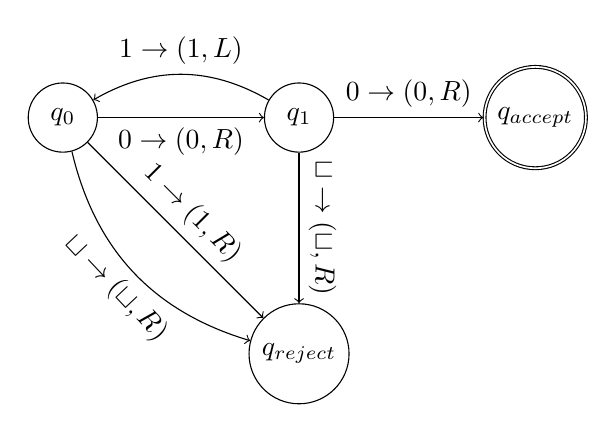
\begin{tikzpicture}[node distance=3cm,on grid,auto]
    \node[state] (q0) at (0,0) {$q_0$};
    \node[state] (q1) [right of=q0] {$q_1$};
    \node[accepting,state] (qaccept) [right of=q1] {$q_{accept}$};
    \node[state] (qreject) [below of=q1] {$q_{reject}$};
    \path[->]
        (q0) edge[anchor=north] node {$0 \to (0, R)$} (q1)
        (q1) edge node {$0 \to (0, R)$} (qaccept)
        (q0) edge node[sloped, anchor=south] {$1 \to (1, R)$} (qreject)
        (q0) edge[bend right, sloped, anchor=north] node {$\sqcup \to (\sqcup, R)$} (qreject)
        (q1) edge[bend right, anchor=south] node {$1 \to (1, L)$} (q0)
        (q1) edge[sloped, anchor=south] node {$\sqcup \to (\sqcup, R)$} (qreject);
\end{tikzpicture}
\end{center}

Question: Does $M$ accept or reject $01$?
\end{frame}

\begin{frame}[noframenumbering]
\frametitle{Quiz Time!}

\begin{center}
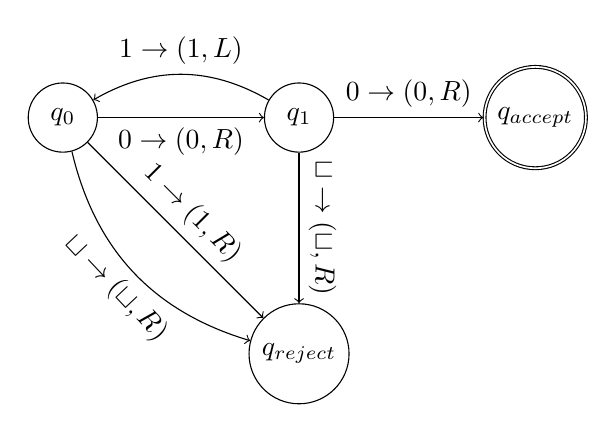
\begin{tikzpicture}[node distance=3cm,on grid,auto]
    \node[state] (q0) at (0,0) {$q_0$};
    \node[state] (q1) [right of=q0] {$q_1$};
    \node[accepting,state] (qaccept) [right of=q1] {$q_{accept}$};
    \node[state] (qreject) [below of=q1] {$q_{reject}$};
    \path[->]
        (q0) edge[anchor=north] node {$0 \to (0, R)$} (q1)
        (q1) edge node {$0 \to (0, R)$} (qaccept)
        (q0) edge node[sloped, anchor=south] {$1 \to (1, R)$} (qreject)
        (q0) edge[bend right, sloped, anchor=north] node {$\sqcup \to (\sqcup, R)$} (qreject)
        (q1) edge[bend right, anchor=south] node {$1 \to (1, L)$} (q0)
        (q1) edge[sloped, anchor=south] node {$\sqcup \to (\sqcup, R)$} (qreject);
\end{tikzpicture}
\end{center}

Answer: $M$ doesn't halt on $01$.
\end{frame}

\begin{frame}
\frametitle{The halting problem}
You might think it would be useful if we could tell when a machine was going to halt.

Formally, we want a $TM\, H$ such that given $TM\, M \text{ and } w \in \Sigma_M^*$:

\begin{itemize}
    \item $H$ halts in the accept state if $M$ halts on $w$ and
    \item $H$ halts in the reject state if $M$ does not halt on $w$.
\end{itemize}

\end{frame}

\begin{frame}
\frametitle{The halting problem}

Assume $H$ exists. Let's build another machine $H'$ which starts with a machine $M$ on its tape.

$H'$ is described as follows:
\begin{algorithm}[H]
\eIf{$H$ accepts $(M, M)$}{go into an infinite loop}
{accept}
\end{algorithm}

What happens if we run $H'$ on $H'$?

\end{frame}

\begin{frame}
\frametitle{The halting problem}

$H$ cannot determine whether or not $H'$ halts on $H'$, so it is impossible to define a machine that halts on every input.

There are many other unsolvable problems as well within the area of {\bf computability theory}. We will not cover this area, but some reading on the subject is suggested at the end.

\end{frame}

\begin{frame}
\frametitle{The reject state}

The reject state is often defined implicitly for convenience.

For any state except the accept state that doesn't have transitions for every symbol in the tape alphabet, it is assumed that there is a transition to the reject state.

\begin{center}
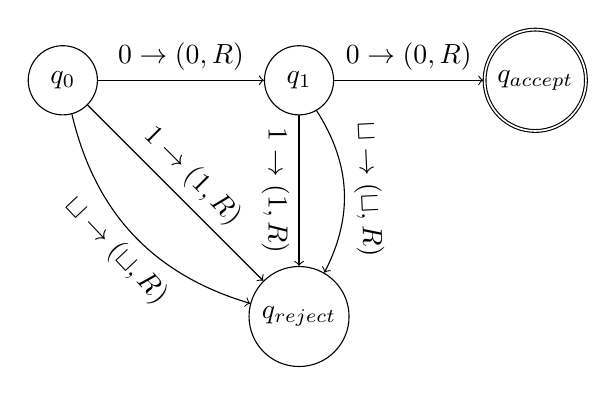
\begin{tikzpicture}[node distance=3cm,on grid,auto]
    \node[state] (q0) at (0,0) {$q_0$};
    \node[state] (q1) [right of=q0] {$q_1$};
    \node[accepting,state] (qaccept) [right of=q1] {$q_{accept}$};
    \node[state] (qreject) [below of=q1] {$q_{reject}$};
    \path[->]
        (q0) edge node {$0 \to (0, R)$} (q1)
        (q1) edge node {$0 \to (0, R)$} (qaccept)
        (q0) edge node[sloped, anchor=south] {$1 \to (1, R)$} (qreject)
        (q0) edge[bend right, sloped, anchor=north] node {$\sqcup \to (\sqcup, R)$} (qreject)
        (q1) edge node[sloped, anchor=north] {$1 \to (1, R)$} (qreject)
        (q1) edge[bend left, sloped, anchor=south] node {$\sqcup \to (\sqcup, R)$} (qreject);
\end{tikzpicture}
\end{center}
\end{frame}

\begin{frame}[noframenumbering]
\frametitle{The reject state}

The reject state is often defined implicitly for convenience.

For any state except the accept state that doesn't have transitions for every symbol in the tape alphabet, it is assumed that there is a transition to the reject state.

\begin{center}
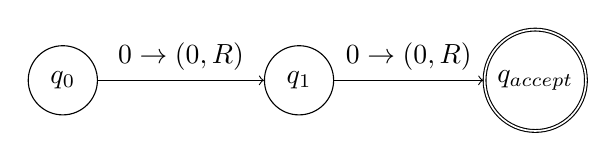
\begin{tikzpicture}[node distance=3cm,on grid,auto]
    \node[state] (q0) at (0,0) {$q_0$};
    \node[state] (q1) [right of=q0] {$q_1$};
    \node[accepting,state] (qaccept) [right of=q1] {$q_{accept}$};
    \path[->]
        (q0) edge node {$0 \to (0, R)$} (q1)
        (q1) edge node {$0 \to (0, R)$} (qaccept);
\end{tikzpicture}
\end{center}
\end{frame}

\begin{frame}
\frametitle{Nondeterminism: Spot the difference!}
A Nondeterministic Turing Machine $(NTM)$ is specified as a tuple of seven components $(Q, \Sigma, \Gamma, q_0, q_{accept}, q_{reject}, \delta)$:

\begin{itemize}
    \item<1-> $Q$ is the set of all possible states
    \item<2-> $\Sigma$ is the input alphabet for the tape. Note that $\Sigma$ cannot contain the blank symbol $\sqcup$
    \item<3-> $\Gamma$ is tape alphabet, where $\Sigma \subseteq \Gamma$ and $\sqcup \in \Gamma$
    \item<4-> $q_0 \in Q$ is the start state
    \item<5-> $q_{accept} \in Q$ is the accept state
    \item<6-> $q_{reject} \in Q$ is the reject state, where $q_{reject} \neq q_{accept}$
    \item<7-> $\delta: Q \times \Gamma \to (Q \times \Sigma \times \{L, R\})^+$ is the transition function
\end{itemize}
\end{frame}

\begin{frame}
\frametitle{What, what's the difference?}
$NTM$s are different because of the transition function.

In deterministic $TMs$, the transition goes from one machine setup to another.

In $NTM$s, the transition function goes from one to many setups.

These setups are run simultaneously, and the machine accepts if one setup halts in an accepting state, or rejects if all setups halt in the rejecting state.

\begin{center}
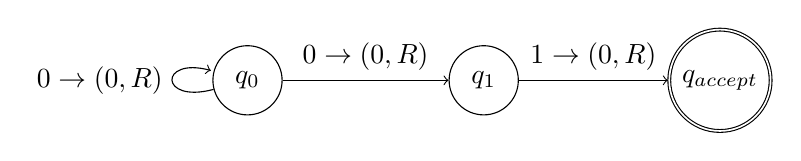
\begin{tikzpicture}[node distance=3cm,on grid,auto]
    \node[state] (q0) at (0,0) {$q_0$};
    \node[state] (q1) [right of=q0] {$q_1$};
    \node[accepting,state] (qaccept) [right of=q1] {$q_{accept}$};
    \path[->]
        (q0) edge node {$0 \to (0, R)$} (q1)
        (q0) edge[loop left] node {$0 \to (0, R)$} (q0)
        (q1) edge node {$1 \to (0, R)$} (qaccept);
\end{tikzpicture}
\end{center}
\end{frame}

\begin{frame}
\frametitle{Computation Tree}
\begin{center}
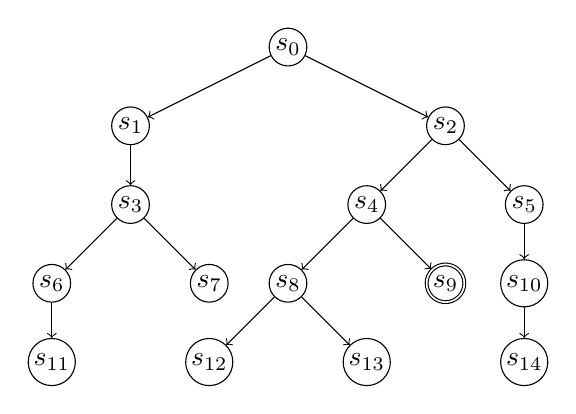
\begin{tikzpicture}
	\tikzset{state/.append style={inner sep=1pt,minimum size=0pt}}
	\node[state] (s0) at (0,0) {$s_0$};
	\node[state] (s1) at (-2,-1) {$s_1$};
	\node[state] (s2) at (2,-1) {$s_2$};
	\node[state] (s3) at (-2,-2) {$s_3$};
	\node[state] (s4) at (1,-2) {$s_4$};
	\node[state] (s5) at (3,-2) {$s_5$};
	\node[state] (s6) at (-3,-3) {$s_6$};
	\node[state] (s7) at (-1,-3) {$s_7$};
	\node[state] (s8) at (0,-3) {$s_8$};
	\node[state, accepting] (s9) at (2,-3) {$s_9$};
	\node[state] (s10) at (3,-3) {$s_{10}$};
	\node[state] (s11) at (-3,-4) {$s_{11}$};
	\node[state] (s12) at (-1,-4) {$s_{12}$};
	\node[state] (s13) at (1,-4) {$s_{13}$};
	\node[state] (s14) at (3,-4) {$s_{14}$};
	\path[->]
		(s0) edge node {} (s1)
		(s0) edge node {} (s2)
		(s1) edge node {} (s3)
		(s2) edge node {} (s4)
		(s2) edge node {} (s5)
		(s3) edge node {} (s6)
		(s3) edge node {} (s7)
		(s4) edge node {} (s8)
		(s4) edge node {} (s9)
		(s5) edge node {} (s10)
		(s6) edge node {} (s11)
		(s8) edge node {} (s12)
		(s8) edge node {} (s13)
		(s10) edge node {} (s14);
\end{tikzpicture}
\end{center}

Vertices are single setups (current state, tape contents and head position) for an $NTM$ running on an input $w \in \Sigma^*$. Edges are transitions.
\end{frame}

\begin{frame}
\frametitle{Power of Nondeterminism}
Any $TM$ is by definition also an $NTM$. The computation tree for a $TM$ looks like this:
\begin{center}
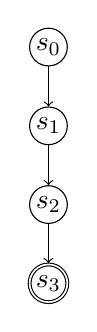
\begin{tikzpicture}
	\tikzset{state/.append style={inner sep=1pt,minimum size=0pt}}
	\node[state] (s0) at (0,0) {$s_0$};
	\node[state] (s1) at (0,-1) {$s_1$};
	\node[state] (s2) at (0,-2) {$s_2$};
	\node[state, accepting] (s3) at (0,-3) {$s_3$};
	\path[->]
		(s0) edge node {} (s1)
		(s1) edge node {} (s2)
		(s2) edge node {} (s3);
\end{tikzpicture}
\end{center}

Question: Is there any problem that can be solved by an $NTM$ that cannot be solved by a $TM$?
\end{frame}

\begin{frame}
\frametitle{Using $TM$s to simulate $NTM$s}
\begin{center}
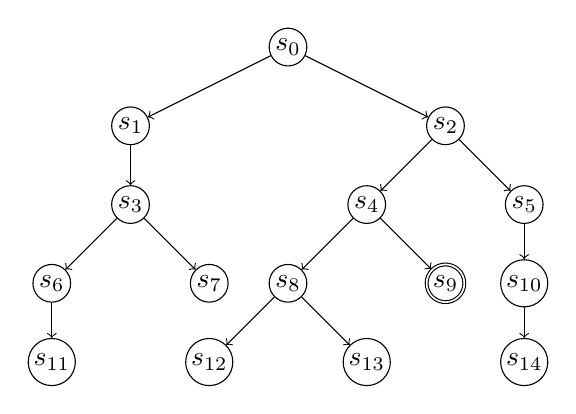
\begin{tikzpicture}
	\tikzset{state/.append style={inner sep=1pt,minimum size=0pt}}
	\node[state] (s0) at (0,0) {$s_0$};
	\node[state] (s1) at (-2,-1) {$s_1$};
	\node[state] (s2) at (2,-1) {$s_2$};
	\node[state] (s3) at (-2,-2) {$s_3$};
	\node[state] (s4) at (1,-2) {$s_4$};
	\node[state] (s5) at (3,-2) {$s_5$};
	\node[state] (s6) at (-3,-3) {$s_6$};
	\node[state] (s7) at (-1,-3) {$s_7$};
	\node[state] (s8) at (0,-3) {$s_8$};
	\node[state, accepting] (s9) at (2,-3) {$s_9$};
	\node[state] (s10) at (3,-3) {$s_{10}$};
	\node[state] (s11) at (-3,-4) {$s_{11}$};
	\node[state] (s12) at (-1,-4) {$s_{12}$};
	\node[state] (s13) at (1,-4) {$s_{13}$};
	\node[state] (s14) at (3,-4) {$s_{14}$};
	\path[->]
		(s0) edge node {} (s1)
		(s0) edge node {} (s2)
		(s1) edge node {} (s3)
		(s2) edge node {} (s4)
		(s2) edge node {} (s5)
		(s3) edge node {} (s6)
		(s3) edge node {} (s7)
		(s4) edge node {} (s8)
		(s4) edge node {} (s9)
		(s5) edge node {} (s10)
		(s6) edge node {} (s11)
		(s8) edge node {} (s12)
		(s8) edge node {} (s13)
		(s10) edge node {} (s14);
\end{tikzpicture}
\end{center}

We can use Breadth-First Search\footnote{\url{https://en.wikipedia.org/wiki/Breadth-first_search}} to search the computation tree until we find an accept state.
\end{frame}

\begin{frame}[noframenumbering]
\frametitle{Using $TM$s to simulate $NTM$s}
\begin{center}
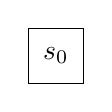
\begin{tikzpicture}
	\edef\sizetape{0.7cm}
	\tikzstyle{tmtape}=[draw,minimum size=\sizetape]

	%% Draw TM tape
	\begin{scope}[shift={(2cm,0cm)},start chain=1 going right,node distance=-0.15mm]
	    \node [on chain=1,tmtape] {$s_0$};
	\end{scope}
\end{tikzpicture}
\end{center}
\end{frame}

\begin{frame}[noframenumbering]
\frametitle{Using $TM$s to simulate $NTM$s}
\begin{center}
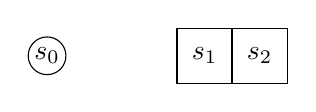
\begin{tikzpicture}
	\tikzset{state/.append style={inner sep=1pt,minimum size=0pt}}
	\node[state] (s0) at (0,0) {$s_0$};

	\edef\sizetape{0.7cm}
	\tikzstyle{tmtape}=[draw,minimum size=\sizetape]

	%% Draw TM tape
	\begin{scope}[shift={(2cm,0cm)},start chain=1 going right,node distance=-0.15mm]
	    \node [on chain=1,tmtape] {$s_1$};
	    \node [on chain=1,tmtape] {$s_2$};
	\end{scope}
\end{tikzpicture}
\end{center}
\end{frame}

\begin{frame}[noframenumbering]
\frametitle{Using $TM$s to simulate $NTM$s}
\begin{center}
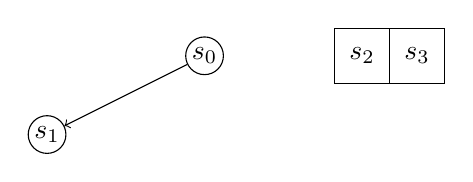
\begin{tikzpicture}
	\tikzset{state/.append style={inner sep=1pt,minimum size=0pt}}
	\node[state] (s0) at (0,0) {$s_0$};
	\node[state] (s1) at (-2,-1) {$s_1$};
	\path[->]
		(s0) edge node {} (s1);

	\edef\sizetape{0.7cm}
	\tikzstyle{tmtape}=[draw,minimum size=\sizetape]

	%% Draw TM tape
	\begin{scope}[shift={(2cm,0cm)},start chain=1 going right,node distance=-0.15mm]
	    \node [on chain=1,tmtape] {$s_2$};
	    \node [on chain=1,tmtape] {$s_3$};
	\end{scope}
\end{tikzpicture}
\end{center}
\end{frame}

\begin{frame}[noframenumbering]
\frametitle{Using $TM$s to simulate $NTM$s}
\begin{center}
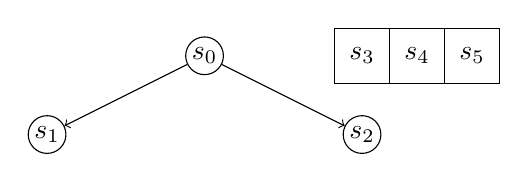
\begin{tikzpicture}
	\tikzset{state/.append style={inner sep=1pt,minimum size=0pt}}
	\node[state] (s0) at (0,0) {$s_0$};
	\node[state] (s1) at (-2,-1) {$s_1$};
	\node[state] (s2) at (2,-1) {$s_2$};
	\path[->]
		(s0) edge node {} (s1)
		(s0) edge node {} (s2);

	\edef\sizetape{0.7cm}
	\tikzstyle{tmtape}=[draw,minimum size=\sizetape]

	%% Draw TM tape
	\begin{scope}[shift={(2cm,0cm)},start chain=1 going right,node distance=-0.15mm]
	    \node [on chain=1,tmtape] {$s_3$};
	    \node [on chain=1,tmtape] {$s_4$};
	    \node [on chain=1,tmtape] {$s_5$};
	\end{scope}
\end{tikzpicture}
\end{center}
\end{frame}

\begin{frame}[noframenumbering]
\frametitle{Using $TM$s to simulate $NTM$s}
\begin{center}
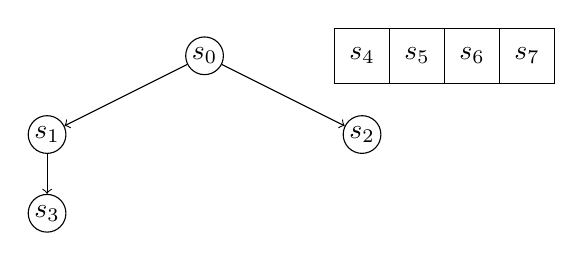
\begin{tikzpicture}
	\tikzset{state/.append style={inner sep=1pt,minimum size=0pt}}
	\node[state] (s0) at (0,0) {$s_0$};
	\node[state] (s1) at (-2,-1) {$s_1$};
	\node[state] (s2) at (2,-1) {$s_2$};
	\node[state] (s3) at (-2,-2) {$s_3$};
	\path[->]
		(s0) edge node {} (s1)
		(s0) edge node {} (s2)
		(s1) edge node {} (s3);

	\edef\sizetape{0.7cm}
	\tikzstyle{tmtape}=[draw,minimum size=\sizetape]

	%% Draw TM tape
	\begin{scope}[shift={(2cm,0cm)},start chain=1 going right,node distance=-0.15mm]
	    \node [on chain=1,tmtape] {$s_4$};
	    \node [on chain=1,tmtape] {$s_5$};
	    \node [on chain=1,tmtape] {$s_6$};
	    \node [on chain=1,tmtape] {$s_7$};
	\end{scope}
\end{tikzpicture}
\end{center}
\end{frame}

\begin{frame}[noframenumbering]
\frametitle{Using $TM$s to simulate $NTM$s}
\begin{center}
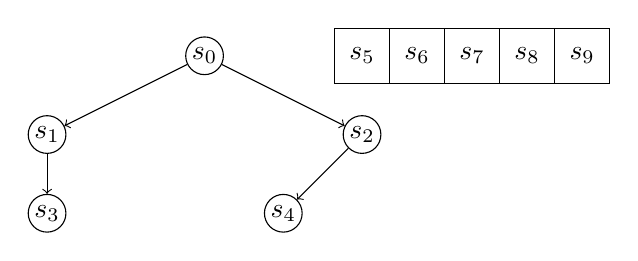
\begin{tikzpicture}
	\tikzset{state/.append style={inner sep=1pt,minimum size=0pt}}
	\node[state] (s0) at (0,0) {$s_0$};
	\node[state] (s1) at (-2,-1) {$s_1$};
	\node[state] (s2) at (2,-1) {$s_2$};
	\node[state] (s3) at (-2,-2) {$s_3$};
	\node[state] (s4) at (1,-2) {$s_4$};
	\path[->]
		(s0) edge node {} (s1)
		(s0) edge node {} (s2)
		(s1) edge node {} (s3)
		(s2) edge node {} (s4);

	\edef\sizetape{0.7cm}
	\tikzstyle{tmtape}=[draw,minimum size=\sizetape]

	%% Draw TM tape
	\begin{scope}[shift={(2cm,0cm)},start chain=1 going right,node distance=-0.15mm]
	    \node [on chain=1,tmtape] {$s_5$};
	    \node [on chain=1,tmtape] {$s_6$};
	    \node [on chain=1,tmtape] {$s_7$};
	    \node [on chain=1,tmtape] {$s_8$};
	    \node [on chain=1,tmtape] {$s_9$};
	\end{scope}
\end{tikzpicture}
\end{center}
\end{frame}

\begin{frame}[noframenumbering]
\frametitle{Using $TM$s to simulate $NTM$s}
\begin{center}
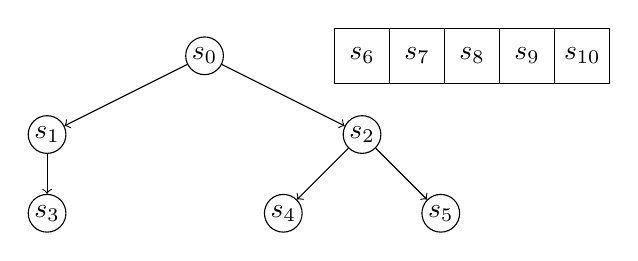
\begin{tikzpicture}
	\tikzset{state/.append style={inner sep=1pt,minimum size=0pt}}
	\node[state] (s0) at (0,0) {$s_0$};
	\node[state] (s1) at (-2,-1) {$s_1$};
	\node[state] (s2) at (2,-1) {$s_2$};
	\node[state] (s3) at (-2,-2) {$s_3$};
	\node[state] (s4) at (1,-2) {$s_4$};
	\node[state] (s5) at (3,-2) {$s_5$};
	\path[->]
		(s0) edge node {} (s1)
		(s0) edge node {} (s2)
		(s1) edge node {} (s3)
		(s2) edge node {} (s4)
		(s2) edge node {} (s5);

	\edef\sizetape{0.7cm}
	\tikzstyle{tmtape}=[draw,minimum size=\sizetape]

	%% Draw TM tape
	\begin{scope}[shift={(2cm,0cm)},start chain=1 going right,node distance=-0.15mm]
	    \node [on chain=1,tmtape] {$s_6$};
	    \node [on chain=1,tmtape] {$s_7$};
	    \node [on chain=1,tmtape] {$s_8$};
	    \node [on chain=1,tmtape] {$s_9$};
	    \node [on chain=1,tmtape] {$s_{10}$};
	\end{scope}
\end{tikzpicture}
\end{center}
\end{frame}

\begin{frame}[noframenumbering]
\frametitle{Using $TM$s to simulate $NTM$s}
\begin{center}
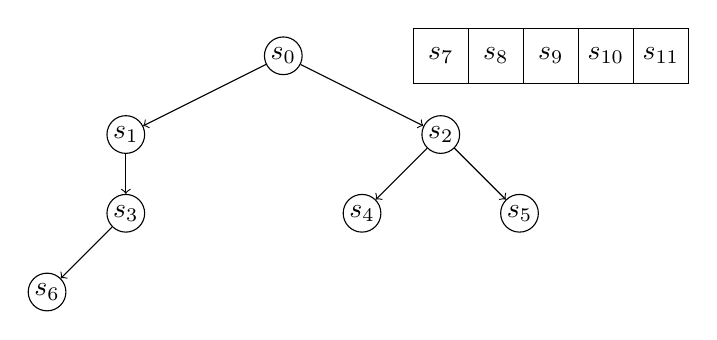
\begin{tikzpicture}
	\tikzset{state/.append style={inner sep=1pt,minimum size=0pt}}
	\node[state] (s0) at (0,0) {$s_0$};
	\node[state] (s1) at (-2,-1) {$s_1$};
	\node[state] (s2) at (2,-1) {$s_2$};
	\node[state] (s3) at (-2,-2) {$s_3$};
	\node[state] (s4) at (1,-2) {$s_4$};
	\node[state] (s5) at (3,-2) {$s_5$};
	\node[state] (s6) at (-3,-3) {$s_6$};
	\path[->]
		(s0) edge node {} (s1)
		(s0) edge node {} (s2)
		(s1) edge node {} (s3)
		(s2) edge node {} (s4)
		(s2) edge node {} (s5)
		(s3) edge node {} (s6);

	\edef\sizetape{0.7cm}
	\tikzstyle{tmtape}=[draw,minimum size=\sizetape]

	%% Draw TM tape
	\begin{scope}[shift={(2cm,0cm)},start chain=1 going right,node distance=-0.15mm]
	    \node [on chain=1,tmtape] {$s_7$};
	    \node [on chain=1,tmtape] {$s_8$};
	    \node [on chain=1,tmtape] {$s_9$};
	    \node [on chain=1,tmtape] {$s_{10}$};
	    \node [on chain=1,tmtape] {$s_{11}$};
	\end{scope}
\end{tikzpicture}
\end{center}
\end{frame}

\begin{frame}[noframenumbering]
\frametitle{Using $TM$s to simulate $NTM$s}
\begin{center}
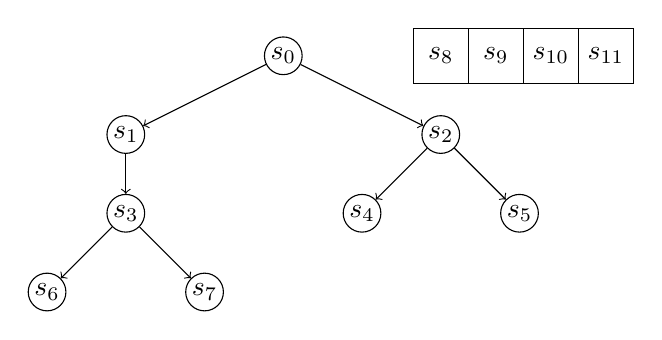
\begin{tikzpicture}
	\tikzset{state/.append style={inner sep=1pt,minimum size=0pt}}
	\node[state] (s0) at (0,0) {$s_0$};
	\node[state] (s1) at (-2,-1) {$s_1$};
	\node[state] (s2) at (2,-1) {$s_2$};
	\node[state] (s3) at (-2,-2) {$s_3$};
	\node[state] (s4) at (1,-2) {$s_4$};
	\node[state] (s5) at (3,-2) {$s_5$};
	\node[state] (s6) at (-3,-3) {$s_6$};
	\node[state] (s7) at (-1,-3) {$s_7$};
	\path[->]
		(s0) edge node {} (s1)
		(s0) edge node {} (s2)
		(s1) edge node {} (s3)
		(s2) edge node {} (s4)
		(s2) edge node {} (s5)
		(s3) edge node {} (s6)
		(s3) edge node {} (s7);

	\edef\sizetape{0.7cm}
	\tikzstyle{tmtape}=[draw,minimum size=\sizetape]

	%% Draw TM tape
	\begin{scope}[shift={(2cm,0cm)},start chain=1 going right,node distance=-0.15mm]
	    \node [on chain=1,tmtape] {$s_8$};
	    \node [on chain=1,tmtape] {$s_9$};
	    \node [on chain=1,tmtape] {$s_{10}$};
	    \node [on chain=1,tmtape] {$s_{11}$};
	\end{scope}
\end{tikzpicture}
\end{center}
\end{frame}

\begin{frame}[noframenumbering]
\frametitle{Using $TM$s to simulate $NTM$s}
\begin{center}
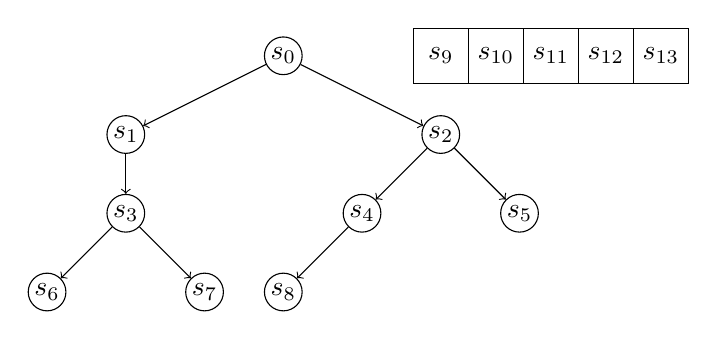
\begin{tikzpicture}
	\tikzset{state/.append style={inner sep=1pt,minimum size=0pt}}
	\node[state] (s0) at (0,0) {$s_0$};
	\node[state] (s1) at (-2,-1) {$s_1$};
	\node[state] (s2) at (2,-1) {$s_2$};
	\node[state] (s3) at (-2,-2) {$s_3$};
	\node[state] (s4) at (1,-2) {$s_4$};
	\node[state] (s5) at (3,-2) {$s_5$};
	\node[state] (s6) at (-3,-3) {$s_6$};
	\node[state] (s7) at (-1,-3) {$s_7$};
	\node[state] (s8) at (0,-3) {$s_8$};
	\path[->]
		(s0) edge node {} (s1)
		(s0) edge node {} (s2)
		(s1) edge node {} (s3)
		(s2) edge node {} (s4)
		(s2) edge node {} (s5)
		(s3) edge node {} (s6)
		(s3) edge node {} (s7)
		(s4) edge node {} (s8);

	\edef\sizetape{0.7cm}
	\tikzstyle{tmtape}=[draw,minimum size=\sizetape]

	%% Draw TM tape
	\begin{scope}[shift={(2cm,0cm)},start chain=1 going right,node distance=-0.15mm]
	    \node [on chain=1,tmtape] {$s_9$};
	    \node [on chain=1,tmtape] {$s_{10}$};
	    \node [on chain=1,tmtape] {$s_{11}$};
	    \node [on chain=1,tmtape] {$s_{12}$};
	    \node [on chain=1,tmtape] {$s_{13}$};
	\end{scope}
\end{tikzpicture}
\end{center}
\end{frame}

\begin{frame}[noframenumbering]
\frametitle{Using $TM$s to simulate $NTM$s}
\begin{center}
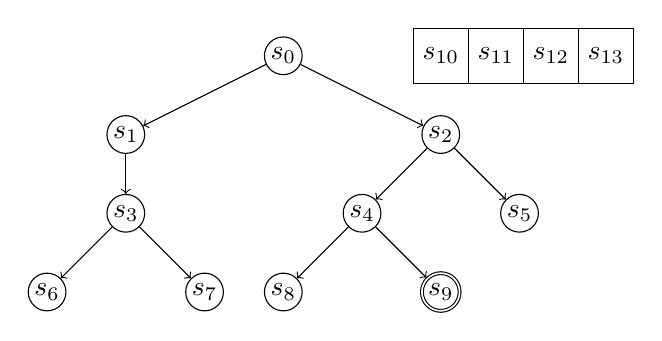
\begin{tikzpicture}
	\tikzset{state/.append style={inner sep=1pt,minimum size=0pt}}
	\node[state] (s0) at (0,0) {$s_0$};
	\node[state] (s1) at (-2,-1) {$s_1$};
	\node[state] (s2) at (2,-1) {$s_2$};
	\node[state] (s3) at (-2,-2) {$s_3$};
	\node[state] (s4) at (1,-2) {$s_4$};
	\node[state] (s5) at (3,-2) {$s_5$};
	\node[state] (s6) at (-3,-3) {$s_6$};
	\node[state] (s7) at (-1,-3) {$s_7$};
	\node[state] (s8) at (0,-3) {$s_8$};
	\node[state, accepting] (s9) at (2,-3) {$s_9$};
	\path[->]
		(s0) edge node {} (s1)
		(s0) edge node {} (s2)
		(s1) edge node {} (s3)
		(s2) edge node {} (s4)
		(s2) edge node {} (s5)
		(s3) edge node {} (s6)
		(s3) edge node {} (s7)
		(s4) edge node {} (s8)
		(s4) edge node {} (s9);

	\edef\sizetape{0.7cm}
	\tikzstyle{tmtape}=[draw,minimum size=\sizetape]

	%% Draw TM tape
	\begin{scope}[shift={(2cm,0cm)},start chain=1 going right,node distance=-0.15mm]
	    \node [on chain=1,tmtape] {$s_{10}$};
	    \node [on chain=1,tmtape] {$s_{11}$};
	    \node [on chain=1,tmtape] {$s_{12}$};
	    \node [on chain=1,tmtape] {$s_{13}$};
	\end{scope}
\end{tikzpicture}
\end{center}
\end{frame}

\begin{frame}
\frametitle{Structure of part one}
\begin{itemize}
    \item What is a computer? {\em Deterministic Turing Machine, Nondeterministic Turing Machine}
    \item What is a problem?
    \item How do we measure performance?
\end{itemize}
\end{frame}

%------------------------------------------------
\section{What is a problem?}
%------------------------------------------------

\begin{frame}
\frametitle{Describing problems as languages}
A {\em language} $L$ is a (potentially infinite) set.

Example languages:
\begin{itemize}
    \item<1-> Text strings that contain the word ``Hello''
    \item<2-> Satisfiable boolean expressions
    \item<3-> Eulerian graphs
    \item<4-> Hamiltonian graphs
    \item<5-> $(M, w)$ such that $M$ halts when given input $w$
\end{itemize}
\end{frame}

\begin{frame}
\frametitle{Decidable languages}
A language $L$ is {\em decidable} if there exists a machine $M$ such that:

\begin{itemize}
    \item $\forall w \in L, M \text{ accepts } w$
    \item $\forall w \notin L, M \text{ rejects } w$
\end{itemize}
\end{frame}

\begin{frame}
\frametitle{Verifiable languages}
A language $L$ is {\em verifiable} if there exists a machine $V$ such that:

\begin{itemize}
    \item $\forall w \in L, \exists c \in \Sigma^* \text{ s.t. } V \text{ accepts } (w,c)$
    \item $\forall w \notin L, \forall c \in \Sigma^*, V \text{ rejects } (w,c)$
\end{itemize}
\end{frame}

\begin{frame}
\frametitle{Structure of part one}
\begin{itemize}
    \item What is a computer? {\em Deterministic Turing Machine, Nondeterministic Turing Machine}
    \item What is a problem? {\em Deciding if a word is in a language, verifying that a word is in a language}
    \item How do we measure performance?
\end{itemize}
\end{frame}

%------------------------------------------------
\section{How do we measure performance?}
%------------------------------------------------

\begin{frame}
\frametitle{Performance of a machine}
We want to talk about how much time it takes for a machine to solve a problem.

To do this, we'll assume $\delta$ takes a constant amount of time to run and count the number of times we call $\delta$.

To remain general, we will focus on how the number of times we call $\delta$ scales in the worst case as the input becomes larger.

We can represent this time complexity as a function of the size of the input.
\end{frame}

\begin{frame}
\frametitle{Problem: Time complexity might be complicated to work out}
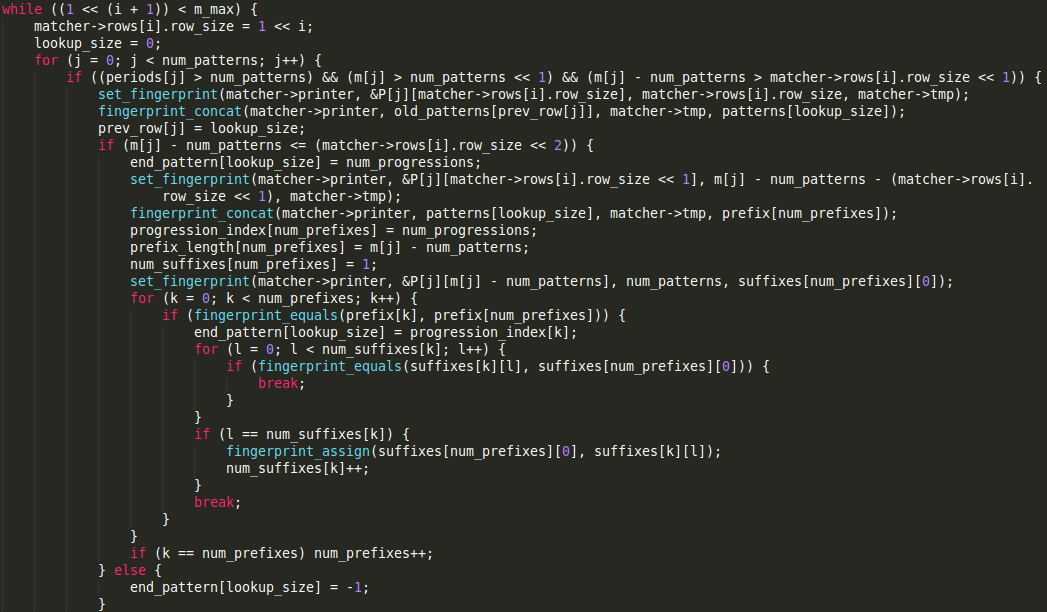
\includegraphics[scale=0.25]{complex_code}\footnote{\url{https://github.com/djmylt/dict_matching/blob/master/dict_matching.h}}
\end{frame}

\begin{frame}
\frametitle{Solution: Approximate!}
Let $f$ and $g$ be functions over the real numbers. We say that:

\begin{itemize}
\item<1->$f(n) \in O(g(n)) \text{ iff } \exists c > 0, n_0 \geq 0 \text{ s.t. } \forall n \geq n_0, f(n) \leq c \cdot g(n)$

\item<2->$f(n) \in \Omega(g(n)) \text{ iff } \exists c > 0, n_0 \geq 0 \text{ s.t. } \forall n \geq n_0, f(n) \geq c \cdot g(n)$

\item<3->$f(n) \in \Theta(g(n)) \text{ iff } \exists c_1, c_2 > 0, n_0 \geq 0 \text{ s.t. } \forall n \geq n_0, c_1 \cdot g(n) \leq f(n) \leq c_2 \cdot g(n)$
\end{itemize}

We use this notation, called {\em Big-O}, {\em Big-Omega} and {\em Big-Theta}, to simplify our complexity functions by rounding up for upper bounds (Big-O) and down for lower bounds (Big-Omega).
\end{frame}

\begin{frame}
\frametitle{Examples}
We can use the definitions from before to prove each of the following statements:

$$n \in O(n^2)$$
$$2^n \in \Omega(n^2)$$
$$n \in \Theta(2n)$$
\end{frame}

\begin{frame}[noframenumbering]
\frametitle{Examples}
We can use the definitions from before to prove each of the following statements:

$$n \in O(n^2): c = 1, n_0 = 0$$
$$2^n \in \Omega(n^2)$$
$$n \in \Theta(2n)$$
\end{frame}

\begin{frame}[noframenumbering]
\frametitle{Examples}
We can use the definitions from before to prove each of the following statements:

$$n \in O(n^2): c = 1, n_0 = 0$$
$$2^n \in \Omega(n^2): c = 1, n_0 = 0$$
$$n \in \Theta(2n)$$
\end{frame}

\begin{frame}[noframenumbering]
\frametitle{Examples}
We can use the definitions from before to prove each of the following statements:

$$n \in O(n^2): c = 1, n_0 = 0$$
$$2^n \in \Omega(n^2): c = 1, n_0 = 0$$
$$n \in \Theta(2n): c_1 = 0.5, c_2 = 1, n_0 = 0$$
\end{frame}

%------------------------------------------------
\section{Summary of part one}
%------------------------------------------------

\begin{frame}
\frametitle{Summary of part one}
\begin{itemize}
    \item What is a computer? {\em Deterministic Turing Machine, Nondeterministic Turing Machine}
    \item What is a problem? {\em Deciding if a word is in a language, verifying that a word is in a language}
    \item How do we measure performance? {\em Upper bound of time for an input of length $n$}
\end{itemize}
\end{frame}

%------------------------------------------------
\section{End of part one}
%------------------------------------------------

\begin{frame}
\frametitle{End of part one}
\begin{center}
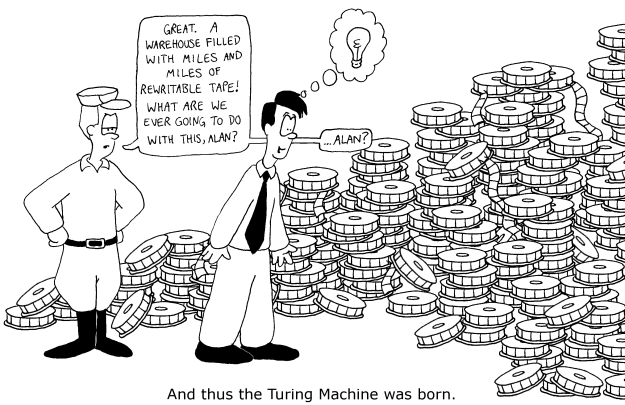
\includegraphics{turing_comic}\footnote{\url{http://www.cs.utah.edu/~draperg/cartoons/2005/turing.html}}
\end{center}
\end{frame}

%------------------------------------------------
\section{Structure of part two}
%------------------------------------------------

\begin{frame}
\frametitle{Structure of part two}
\begin{itemize}
    \item Putting it all together!
    \item ...only to get another (very difficult) problem.
    \item How might we try to solve this new problem?
\end{itemize}
\end{frame}

%------------------------------------------------
\section{Complexity classes}
%------------------------------------------------

\begin{frame}
\frametitle{Complexity Classes}
Now that we have provided our definitions for a computer, a problem and performance, we can look at what problems can be solved under these restrictions.

These are called {\em complexity classes}.
\end{frame}

\begin{frame}
\frametitle{Time Complexity Classes}
Let $t: \mathbb{N} \to \mathbb{R}$ be a function.

$\mathrm{TIME}(t(n))$ is all the languages that can be decided by a $TM$ in $O(t(n))$ time.

$\mathrm{NTIME}(t(n))$ is all the languages that can be decided by a $NTM$ in $O(t(n))$ time.
\end{frame}

\begin{frame}
\frametitle{Deterministic polynomial time}
One example of a complexity class is the set of languages that can be decided by a $TM$ in polynomial time.

$$\bigcup_{k = 0}^{\infty} \mathrm{TIME}(n^k)$$

We shall refer to the set of these problems as $P$.
\end{frame}

\begin{frame}
\frametitle{Nondeterministic polynomial time}
Another example is the set of languages that can be decided by a $NTM$ in polynomial time.

$$\bigcup_{k = 0}^{\infty} \mathrm{NTIME}(n^k)$$

We shall refer to the set of these problems as $NP$.

We can also define $NP$ as the set of languages that can be verified by a $TM$ in polynomial time.
\end{frame}

\begin{frame}
\frametitle{From nondeterminism to verification}
Recall the computation tree for an $NTM$.
\begin{center}
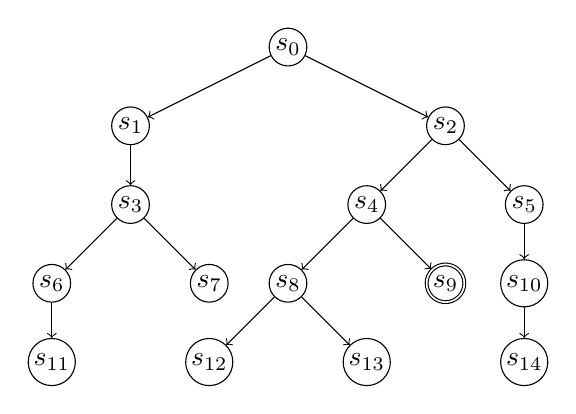
\begin{tikzpicture}
	\tikzset{state/.append style={inner sep=1pt,minimum size=0pt}}
	\node[state] (s0) at (0,0) {$s_0$};
	\node[state] (s1) at (-2,-1) {$s_1$};
	\node[state] (s2) at (2,-1) {$s_2$};
	\node[state] (s3) at (-2,-2) {$s_3$};
	\node[state] (s4) at (1,-2) {$s_4$};
	\node[state] (s5) at (3,-2) {$s_5$};
	\node[state] (s6) at (-3,-3) {$s_6$};
	\node[state] (s7) at (-1,-3) {$s_7$};
	\node[state] (s8) at (0,-3) {$s_8$};
	\node[state, accepting] (s9) at (2,-3) {$s_9$};
	\node[state] (s10) at (3,-3) {$s_{10}$};
	\node[state] (s11) at (-3,-4) {$s_{11}$};
	\node[state] (s12) at (-1,-4) {$s_{12}$};
	\node[state] (s13) at (1,-4) {$s_{13}$};
	\node[state] (s14) at (3,-4) {$s_{14}$};
	\path[->]
		(s0) edge node {} (s1)
		(s0) edge node {} (s2)
		(s1) edge node {} (s3)
		(s2) edge node {} (s4)
		(s2) edge node {} (s5)
		(s3) edge node {} (s6)
		(s3) edge node {} (s7)
		(s4) edge node {} (s8)
		(s4) edge node {} (s9)
		(s5) edge node {} (s10)
		(s6) edge node {} (s11)
		(s8) edge node {} (s12)
		(s8) edge node {} (s13)
		(s10) edge node {} (s14);
\end{tikzpicture}
\end{center}

We label each branch with an integer such that the labels are unique between siblings.
\end{frame}

\begin{frame}[noframenumbering]
\frametitle{From nondeterminism to verification}
Recall the computation tree for an $NTM$.
\begin{center}
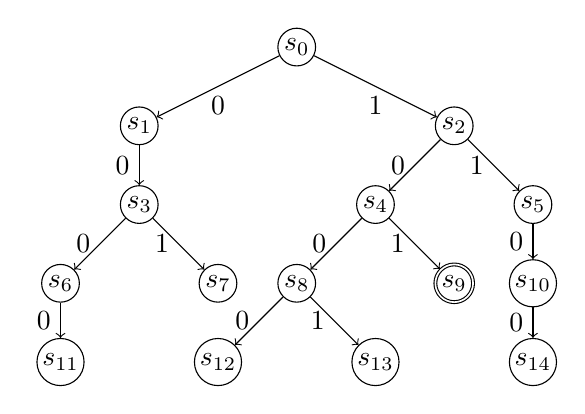
\begin{tikzpicture}
	\tikzset{state/.append style={inner sep=1pt,minimum size=0pt}}
	\node[state] (s0) at (0,0) {$s_0$};
	\node[state] (s1) at (-2,-1) {$s_1$};
	\node[state] (s2) at (2,-1) {$s_2$};
	\node[state] (s3) at (-2,-2) {$s_3$};
	\node[state] (s4) at (1,-2) {$s_4$};
	\node[state] (s5) at (3,-2) {$s_5$};
	\node[state] (s6) at (-3,-3) {$s_6$};
	\node[state] (s7) at (-1,-3) {$s_7$};
	\node[state] (s8) at (0,-3) {$s_8$};
	\node[state, accepting] (s9) at (2,-3) {$s_9$};
	\node[state] (s10) at (3,-3) {$s_{10}$};
	\node[state] (s11) at (-3,-4) {$s_{11}$};
	\node[state] (s12) at (-1,-4) {$s_{12}$};
	\node[state] (s13) at (1,-4) {$s_{13}$};
	\node[state] (s14) at (3,-4) {$s_{14}$};
	\path[->]
		(s0) edge [anchor=north] node {0} (s1)
		(s0) edge [anchor=north] node {1} (s2)
		(s1) edge [anchor=east] node {0} (s3)
		(s2) edge [anchor=east] node {0} (s4)
		(s2) edge [anchor=east] node {1} (s5)
		(s3) edge [anchor=east] node {0} (s6)
		(s3) edge [anchor=east] node {1} (s7)
		(s4) edge [anchor=east] node {0} (s8)
		(s4) edge [anchor=east] node {1} (s9)
		(s5) edge [anchor=east] node {0} (s10)
		(s6) edge [anchor=east] node {0} (s11)
		(s8) edge [anchor=east] node {0} (s12)
		(s8) edge [anchor=east] node {1} (s13)
		(s10) edge [anchor=east] node {0} (s14);
\end{tikzpicture}
\end{center}

We label each branch with an integer such that the labels are unique between siblings.
\end{frame}

\begin{frame}
\frametitle{From nondeterminism to verification}
Our certificate $c$ is now the polynomial length sequence that leads to the accepting state. In this case $c=101$, as can be verified in polynomial time by following the certificate down the tree:
\begin{center}
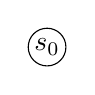
\begin{tikzpicture}
	\tikzset{state/.append style={inner sep=1pt,minimum size=0pt}}
	\node[state] (s0) at (0,0) {$s_0$};
\end{tikzpicture}
\end{center}
\end{frame}

\begin{frame}[noframenumbering]
\frametitle{From nondeterminism to verification}
Our certificate $c$ is now the polynomial length sequence that leads to the accepting state. In this case $c=101$, as can be verified in polynomial time by following the certificate down the tree:
\begin{center}
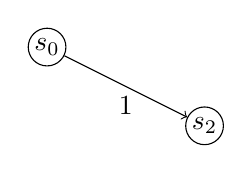
\begin{tikzpicture}
	\tikzset{state/.append style={inner sep=1pt,minimum size=0pt}}
	\node[state] (s0) at (0,0) {$s_0$};
	\node[state] (s2) at (2,-1) {$s_2$};
	\path[->]
		(s0) edge [anchor=north] node {1} (s2);
\end{tikzpicture}
\end{center}
\end{frame}

\begin{frame}[noframenumbering]
\frametitle{From nondeterminism to verification}
Our certificate $c$ is now the polynomial length sequence that leads to the accepting state. In this case $c=101$, as can be verified in polynomial time by following the certificate down the tree:
\begin{center}
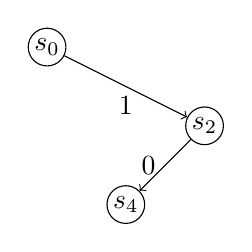
\begin{tikzpicture}
	\tikzset{state/.append style={inner sep=1pt,minimum size=0pt}}
	\node[state] (s0) at (0,0) {$s_0$};
	\node[state] (s2) at (2,-1) {$s_2$};
	\node[state] (s4) at (1,-2) {$s_4$};
	\path[->]
		(s0) edge [anchor=north] node {1} (s2)
		(s2) edge [anchor=east] node {0} (s4);
\end{tikzpicture}
\end{center}
\end{frame}

\begin{frame}[noframenumbering]
\frametitle{From nondeterminism to verification}
Our certificate $c$ is now the polynomial length sequence that leads to the accepting state. In this case $c=101$, as can be verified in polynomial time by following the certificate down the tree:
\begin{center}
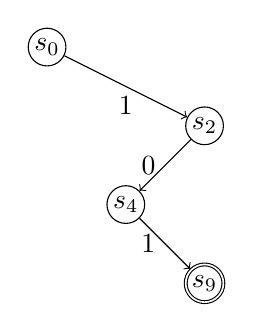
\begin{tikzpicture}
	\tikzset{state/.append style={inner sep=1pt,minimum size=0pt}}
	\node[state] (s0) at (0,0) {$s_0$};
	\node[state] (s2) at (2,-1) {$s_2$};
	\node[state] (s4) at (1,-2) {$s_4$};
	\node[state, accepting] (s9) at (2,-3) {$s_9$};
	\path[->]
		(s0) edge [anchor=north] node {1} (s2)
		(s2) edge [anchor=east] node {0} (s4)
		(s4) edge [anchor=east] node {1} (s9);
\end{tikzpicture}
\end{center}
\end{frame}

\begin{frame}
\frametitle{From verification to nondeterminism}
Since the verifier runs in polynomial time, at most a polynomial number of characters can be read from the certificate.

We use nondeterminism to brute force and verify every certificate of length $k$ for $0 \leq k \leq p(n)$.
\end{frame}

\begin{frame}
\frametitle{From verification to nondeterminism}

The node of the computation tree is the certificate we are verifying at that point.
\begin{center}
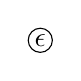
\begin{tikzpicture}
	\tikzset{state/.append style={inner sep=1pt,minimum size=0pt}}
	\node[state] (e) at (0,0) {$\epsilon$};
\end{tikzpicture}
\end{center}
\end{frame}

\begin{frame}[noframenumbering]
\frametitle{From verification to nondeterminism}

The node of the computation tree is the certificate we are verifying at that point.
\begin{center}
\begin{tikzpicture}
	\tikzset{state/.append style={inner sep=1pt,minimum size=0pt}}
	\node[state] (e) at (0,0) {$\epsilon$};
	\node[state] (0) at (-4,-1) {$0$};
	\node[state] (1) at (4,-1) {$1$};
	\path[->]
		(e) edge node {} (0)
		(e) edge node {} (1);
\end{tikzpicture}
\end{center}
\end{frame}

\begin{frame}[noframenumbering]
\frametitle{From verification to nondeterminism}

The node of the computation tree is the certificate we are verifying at that point.
\begin{center}
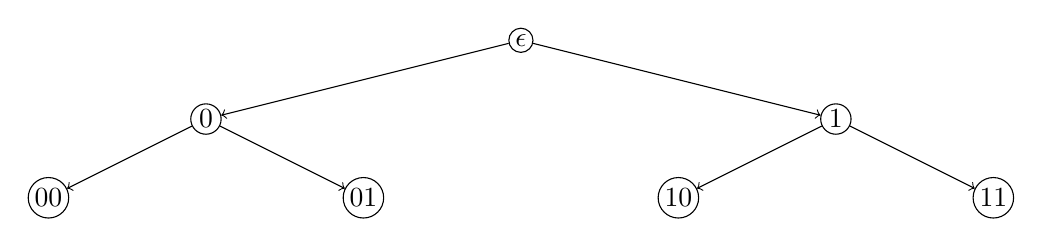
\begin{tikzpicture}
	\tikzset{state/.append style={inner sep=1pt,minimum size=0pt}}
	\node[state] (e) at (0,0) {$\epsilon$};
	\node[state] (0) at (-4,-1) {$0$};
	\node[state] (1) at (4,-1) {$1$};
	\node[state] (00) at (-6,-2) {$00$};
	\node[state] (01) at (-2,-2) {$01$};
	\node[state] (10) at (2,-2) {$10$};
	\node[state] (11) at (6,-2) {$11$};
	\path[->]
		(e) edge node {} (0)
		(e) edge node {} (1)
		(0) edge node {} (00)
		(0) edge node {} (01)
		(1) edge node {} (10)
		(1) edge node {} (11);
\end{tikzpicture}
\end{center}
\end{frame}

\begin{frame}[noframenumbering]
\frametitle{From verification to nondeterminism}

The node of the computation tree is the certificate we are verifying at that point.
\begin{center}
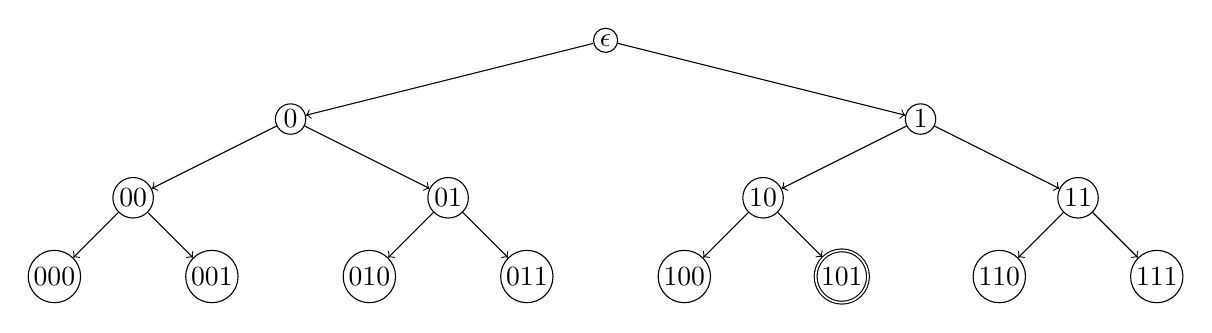
\begin{tikzpicture}
	\tikzset{state/.append style={inner sep=1pt,minimum size=0pt}}
	\node[state] (e) at (0,0) {$\epsilon$};
	\node[state] (0) at (-4,-1) {$0$};
	\node[state] (1) at (4,-1) {$1$};
	\node[state] (00) at (-6,-2) {$00$};
	\node[state] (01) at (-2,-2) {$01$};
	\node[state] (10) at (2,-2) {$10$};
	\node[state] (11) at (6,-2) {$11$};
	\node[state] (000) at (-7,-3) {$000$};
	\node[state] (001) at (-5,-3) {$001$};
	\node[state] (010) at (-3,-3) {$010$};
	\node[state] (011) at (-1,-3) {$011$};
	\node[state] (100) at (1,-3) {$100$};
	\node[state, accepting] (101) at (3,-3) {$101$};
	\node[state] (110) at (5,-3) {$110$};
	\node[state] (111) at (7,-3) {$111$};
	\path[->]
		(e) edge node {} (0)
		(e) edge node {} (1)
		(0) edge node {} (00)
		(0) edge node {} (01)
		(1) edge node {} (10)
		(1) edge node {} (11)
		(00) edge node {} (000)
		(00) edge node {} (001)
		(01) edge node {} (010)
		(01) edge node {} (011)
		(10) edge node {} (100)
		(10) edge node {} (101)
		(11) edge node {} (110)
		(11) edge node {} (111);
\end{tikzpicture}
\end{center}
\end{frame}

\begin{frame}
\frametitle{Structure of part two}
\begin{itemize}
    \item Putting it all together! {\em Complexity classes, $P, NP$}
    \item ...only to get another (very difficult) problem.
    \item How might we try to solve this new problem?
\end{itemize}
\end{frame}

%------------------------------------------------
\section{The $P$ versus $NP$ problem}
%------------------------------------------------

\begin{frame}
\frametitle{Exercise Left For the Student}
\centerline{Does $P=NP$?}
\end{frame}

\begin{frame}
\frametitle{The $P$ versus $NP$ problem}
Arguably first proposed by G\"{o}del in a letter to von Neumann in 1956.\footnote{\url{https://ecommons.cornell.edu/bitstream/handle/1813/6910/89-994.pdf}}

Became known as $P$ versus $NP$ after Cook's work in 1971.

Solving the problem will earn you a million dollars, courtesy of the Clay Mathematics Institute.\footnote{\url{http://www.claymath.org/millennium-problems/p-vs-np-problem}}
\end{frame}

\begin{frame}
\frametitle{The easy side: $P \subseteq NP$}

Recall that any $TM$ is by definition nondeterministic.

Likewise, any polynomial-time $TM$ is also nondeterministic.

Hence $P \subseteq NP$.
\end{frame}

\begin{frame}
\frametitle{The harder side: Is $NP \subseteq P$?}

Another way to think of this problem: {\em If a problem can be easily verified, can it be easily solved?}
\end{frame}

\begin{frame}
\frametitle{Summary of part two}
\begin{itemize}
    \item Putting it all together! {\em Complexity classes, $P, NP$}
    \item ...only to get another (very difficult) problem. {\em Are easy to verify problems easy to solve?}
    \item How might we try to solve this new problem?
\end{itemize}
\end{frame}

%------------------------------------------------
\section{Completeness}
%------------------------------------------------

\begin{frame}
\frametitle{How might we answer this question?}

Why not look at the hardest problems in $NP$?

If $P = NP$, then even the hardest problems in $NP$ will be solvable in polynomial time.

And if $P \subset NP$, then these are the problems that won't have a polynomial time solution, as could be checked by lower-bound analysis.

But how can we determine the hardest problems in $NP$?
\end{frame}

\begin{frame}
\frametitle{Polynomial time computable functions}

A function $f:\Sigma^* \to \Sigma^*$ is polynomial time computable if there exists a polynomial time Turing machine $M$ that, when started with input $w$ on its tape, halts with only $f(w)$ on its tape.

\end{frame}

\begin{frame}
\frametitle{Polynomial time reducible}

Take two languages $A$ and $B$. We say that $A \leq_P B$ if there exists a polynomial time computable function $f$ such that:

\begin{itemize}
    \item $\forall w \in A, f(w) \in B$
    \item $\forall w \notin A, f(w) \notin B$
\end{itemize}

This means that if we have a polynomial time solution for $B$, then we also have a polynomial time solution for $A$.

Note that this property is transitive: If $A \leq_P B \text{ and } B \leq_P C \text{ then } A \leq_P C$

\end{frame}

\begin{frame}
\frametitle{$NP\text{-Complete}$}

A language $B$ is $NP\text{-Complete}$ iff:

\begin{itemize}
    \item $B \in NP$
    \item and $\forall A \in NP, A \leq_P B$
\end{itemize}

If one $NP\text{-Complete}$ language is proven to be in $P$, then every $NP$ problem is also in $P$, so $P$ would be equal to $NP$.
\end{frame}

\begin{frame}
\frametitle{Problem: There are lots of $NP$ problems}
There are an infinite number of $NP$ problems, so it is impossible to provide a reduction to each individual problem.
%Note: Said claim might not be true if you are Jeff Dean, see https://www.quora.com/What-are-all-the-Jeff-Dean-facts
%Note: If you are Jeff Dean, can I have an autograph?

So how can we reduce all of them to a specific problem?
\end{frame}

\begin{frame}
\frametitle{Satisfiable boolean formulae}
Take a boolean formula such as $f = a \vee b \wedge \bar{c}$.

We say that $f$ is {\em satisfiable} (also known as a tautology) if we can assign $\bot$ or $\top$ to each variable such that $f = \top$.

Examples:
\begin{itemize}
    \item $f$ is satisfiable: $(a = \top, b = \top, c =  \bot)$
    \item but $f' = x \wedge \bar{x}$ is not satisfiable
\end{itemize}

We call $SAT$ the language of all satisfiable boolean formulae.
\end{frame}

\begin{frame}
\frametitle{$SAT \in NP$}
$SAT$ can be verified in polynomial time:

\begin{itemize}
    \item<1-> Make the certificate the values we assign to each variable.
    \item<2-> Have $V$ substitute the value for each variable into the formula.
    \item<3-> Accept if the formula evaluates to $\top$, otherwise reject.
\end{itemize}
\end{frame}

\begin{frame}
\frametitle{Cook-Levin Theorem}
Recall that any language in $NP$ can be decided by an $NTM$ in polynomial time.

Cook showed that any $NTM\, M$ that halts in polynomial time running on input $w$ can be converted in polynomial time to a boolean formula such that:

\begin{itemize}
    \item If $M$ accepts $w$, then the formula is satisfiable
    \item and if $M$ rejects $w$, then the formula cannot be satisfied.
\end{itemize}

As a result, it was proven that $SAT \in NP\text{-Complete}$.
\end{frame}

\begin{frame}
\frametitle{Proving other $NP\text{-Complete}$ problems}

Now that we have one $NP\text{-Complete}$ problem, proving others is a lot easier.

Recall that polynomial-time reducibility is transitive.

So now if our problem $B$ is in $NP$ and we can find one problem $A \in NP\text{-Complete}$ such that $A \leq_P B$, then $B \in NP\text{-Complete}$
\end{frame}

\begin{frame}
\frametitle{Other $NP\text{-Complete}$ problems}
\begin{itemize}
    \item<1-> $3SAT$
    \item<2-> Hamiltonian graphs
    \item<3-> Sudokus
    \item<4-> Knapsack
    \item<5-> Tetris
    \item<6-> Super Mario Brothers
    \item<7-> Lemmings
    \item<8-> Bejeweled
    \item<9-> Candy Crush Saga
    \item<10-> Flood-It
\end{itemize}
\end{frame}

%------------------------------------------------
\section{Summary of part two}
%------------------------------------------------

\begin{frame}
\frametitle{Summary of part two}
\begin{itemize}
    \item Putting it all together! {\em Complexity classes, $P, NP$}
    \item ...only to get another (very difficult) problem. {\em Are easy to verify problems easy to solve?}
    \item How might we try to solve this new problem? {\em $NP\text{-Complete}$ problems}
\end{itemize}
\end{frame}

%------------------------------------------------
\section{Beyond $P$ and $NP$}
%------------------------------------------------

\begin{frame}
\frametitle{What else is there?}
Recall our three questions from part one:
\begin{itemize}
    \item What is a computer?
    \item What is a problem?
    \item How do we measure performance?
\end{itemize}
What if we answered these differently?
\end{frame}

\begin{frame}
\frametitle{Different restrictions on time}
Exponential time: $EXP, 2EXP, ELEMENTARY$

Linear time: $LIN$
\end{frame}

\begin{frame}
\frametitle{How do we measure performance?}
Space complexity: $PSPACE, EXPSPACE$

Working space: $L$
\end{frame}

\begin{frame}
\frametitle{What is a problem?}
Computational problems: $NP\text{-Hard}$

Counting problems: $\#P$

Complementary problems: $\text{co-}NP$
\end{frame}

\begin{frame}
\frametitle{What is a computer?}
Probabilistic Turing Machines: $BPP, RP$

Parallel Computing: $NC$

Quantum computers:  $EQP, BQP$

Time travel: $P_{CTC}$
\end{frame}

\begin{frame}
\frametitle{Open problems in complexity theory}
\begin{itemize}
    \item<1-> Does $P = NP$?
    \item<2-> Does $L = NL$?
    \item<3-> Does $BPP = P$?
    \item<4-> Does $BQP = BPP$?
    \item<5-> Does $NC = P$?
    \item<6-> Does $P = PSPACE$?
    \item<7-> Does $NP = \text{co-}NP$?
    \item<8-> And lots more...
\end{itemize}
\end{frame}

\begin{frame}
\frametitle{The Conclusion}
Complexity theory is a large area about what problems are solvable under different models of a computer and different performance requirements.

There are lots of complexity classes out there -- far more than have been mentioned in this presentation -- and very quickly relating them in a simple equation like this:

$$P \subseteq NP$$

Becomes this:

$$L \subseteq NL \subseteq P \subseteq NP \subseteq PSPACE = NPSPACE = P_{CTC} \subseteq EXP \subseteq EXPSPACE$$
\end{frame}

\begin{frame}
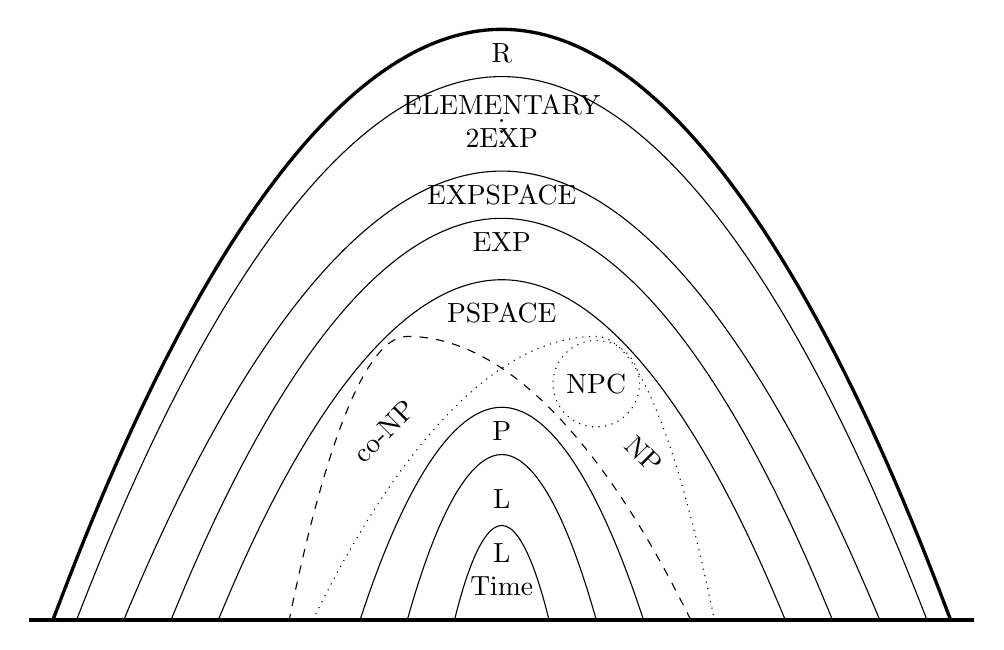
\begin{tikzpicture}
\pgftransformscale{.6}

%%% HELP LINES - uncomment to design/extend
% \draw[step=1cm,gray,very thin] (-10,0) grid (10,12);
% \node at (0,0) {\textbf{(0,0)}};

%% Horizontal bar
\draw[very thick] (10,0) -- (-10,0);

% LOG TIME
\draw (-1,0) parabola bend (0,2) (1,0) ;
\node at (0,1) {
    \begin{tabular}{c}
    L \\ Time
    \end{tabular}
};

% LOG SPACE
\draw (-2,0) parabola bend (0,3.5) (2,0);
\node at (0,2.5) {
    \begin{tabular}{c}
    L
    \end{tabular}
};

% PTIME
\draw (-3,0) parabola bend (0,4.5) (3,0);
\node at (0,4) {P};

% NP
\draw[dotted] (-4,0) parabola bend (2,6) (4.5,0);
\node[rotate=-45] at (3,3.5) {NP};

% NP-complete
\node[circle,dotted,draw] at (2,5) {NPC};

% Co-NP
\draw[dashed] (4,0) parabola bend (-2,6) (-4.5,0);
\node[rotate=45] at (-2.5,4) {co-NP};

% PSPACE
\draw (-6,0) parabola bend (0,7.2) (6,0);
\node at (0,6.5) {PSPACE};

% EXPTIME
\draw (-7,0) parabola bend (0,8.5) (7,0);
\node at (0,8) {EXP};

% EXPTIME
\draw (-8,0) parabola bend (0,9.5) (8,0);
\node at (0,9) {EXPSPACE};

% ELEMENTARY
\draw (-9,0) parabola bend (0,11.5) (9,0);
\node at (0,10.5) {$\vdots$};
\node[anchor=north] at (0,11.4) {
    \begin{tabular}{c}
        ELEMENTARY \\
        2EXP
    \end{tabular}
};

% RECURSIVE
\draw[very thick] (-9.5,0) parabola bend (0,12.5) (9.5,0);
\node at (0,12) {R};
\end{tikzpicture}\footnote{\url{http://www.texample.net/tikz/examples/complexity-classes/}}
\end{frame}

%------------------------------------------------
\section{The end}
%------------------------------------------------

\begin{frame}
\begin{center}
\frametitle{The end}
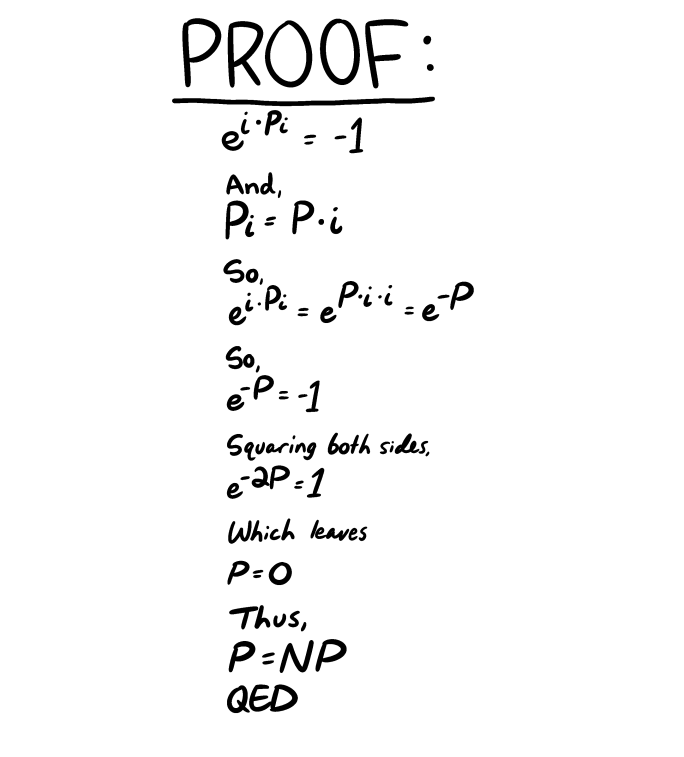
\includegraphics[scale=0.2]{smbc_comic}\footnote{\url{http://www.smbc-comics.com/?id=3919}}
\end{center}
\end{frame}

\begin{frame}
\begin{center}
\frametitle{The end}
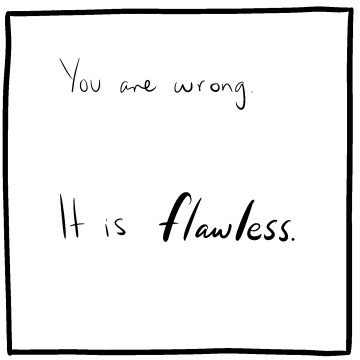
\includegraphics[scale=0.5]{smbc_comic_votey}\footnote{\url{http://www.smbc-comics.com/?id=3919}}
\end{center}
\end{frame}

%------------------------------------------------
\section{Suggested reading}
%------------------------------------------------

\begin{frame}
\frametitle{Suggested books}
\begin{itemize}
    \item {\em Introduction to the Theory of Computation} by Michael Sipser is the recommended textbook for most computability and complexity theory courses
    \item {\em Computers and Intractability: A Guide to the Theory of NP-Completeness} by Michael R.\@ Garey and David S.\@ Johnson covers a lot about $NP\text{-Complete}$ problems, including a very large collection of $NP\text{-Complete}$ problems.
    \item {\em Quantum Computing Since Democritus} by Scott Aaronson offers a broad overview of many complexity classes
\end{itemize}
\end{frame}

\begin{frame}
\frametitle{Suggested papers}
\begin{itemize}
    \item {\em On Computable Numbers, with an Application to the Entscheidungsproblem} by Alan Turing is Turing's PhD thesis, which provides the original definition of Turing Machines, a formal definition of the Universal Turing Machine, and a proof that the Halting problem is undecidable
    \item {\em The Complexity of Theorem Proving Procedures} by Stephen Cook provides the proof that $SAT \in NP\text{-Complete}$
    \item {\em Reducibility Among Combinatorial Problems} by Richard Karp provides 21 of the earliest problems proven to be $NP\text{-Complete}$
\end{itemize}
\end{frame}

\begin{frame}
\frametitle{Suggested websites}
\begin{itemize}
    \item \url{https://complexityzoo.uwaterloo.ca/} is a Wiki originally developed by Scott Aaronson which provides a list of every complexity class ever stated
\end{itemize}
\end{frame}

\begin{frame}
\frametitle{Proofs for $NP\text{-Complete}$ problems}
\begin{itemize}
	\item Takayuki Yato and Takahiro Seta: Complexity and Completeness of Finding Another Solution and Its Application to Puzzles, IEICE TRANSACTIONS on Fundamentals of Electronics, Communications and Computer Sciences, Vol.E86-A, No.5, pp.1052-1060
	\item  Erik D. Demaine, Susan Hohenberger and David Liben-Nowell: Tetris is Hard, Even to Approximate, \url{http://arxiv.org/abs/cs/0210020}
    \item Graham Cormode: The Hardness of the Lemmings Game, or Oh no, more NP-Completeness Proofs, Proceedings of the 3rd International Conference on Fun with Algorithms, May 2004, pages 65-76
    \item Greg Aloupis, Erik D. Demaine, Alan Guo and Giovanni Viglietta: Classic Nintendo Games are (Computationally) Hard, \url{http://arxiv.org/abs/1203.1895}
    \item Luciano Gualà, Stefano Leucci and Emanuele Natale: Bejeweled, Candy Crush and other Match-Three Games are (NP-)Hard, \url{http://arxiv.org/abs/1403.5830}
    \item Rapha\"{e}l Clifford, Markus Jalsenius, Ashley Montanaro and Benjamin Sach:  The Complexity of Flood Filling Games, \url{http://arxiv.org/abs/1001.4420}
\end{itemize}
\end{frame}

\begin{frame}
\frametitle{Post-credits}
\centerline{``You're still here? It's over. Go home. Go.'', {\em Bueller}}
\end{frame}

%----------------------------------------------------------------------------------------

\end{document} 
